\section{Introductory example: dispatch on special matrix types}

We begin with a brief example of how technical programs might combine static
and dynamic dispatch.

\paragraph{Special matrix types}
The Julia base library defines
many specialized matrix types to capture properties
such as triangularity, Hermitianness or bandedness. Many specialized
linear algebra algorithms exist that take advantage of such information.
Furthermore some matrix properties lend themselves to multiple representations.
For example, symmetric matrices may be stored as ordinary matrices, but only
the upper or lower half is ever accessed. Alternatively, they may be stored in
other ways, such as the packed format or rectangular full packed format, which
allow for some faster algorithms, for example, for the Cholesky
factorization~\cite{Gustavson2010}. All three storage formats for symmetric
matrices exist in the LAPACK library for numerical linear algebra; computations
on these formats are distinguished by whether the second and third letters of
the routine's name are \lstinline|SY|, \lstinline|SP| or \lstinline|SF|
respectively. In contrast, Julia's base library contains types like
\lstinline|Symmetric| and \lstinline|SymmetricRFP|, which encode information
about matrix properties and their storage format.

\paragraph{The matrix square root}
Having matrix types like \lstinline|Symmetric| allows Julia programmers to
write code that annotates if a matrix is symmetric. Sometimes, users
will use only symmetric matrices, for example, in code that
works only on adjacency matrices of undirected graphs. In such situations,
it is sensible to construct \lstinline|Symmetric| matrices explictly, as then
Julia can dispatch directly to specialized methods for \lstinline|Symmetric|
types. An example of such a function is \lstinline|sqrtm|, which computes the
principal square root of a matrix. In general, the square root can be computed
via the Schur factorization of a matrix~\cite{Golub2013}. However, the square
root of a \lstinline|Symmetric| matrix can be computed faster and more stably
by diagonalization to find its eigenvalues and
eigenvectors~\cite{Higham2008,Golub2013}. Hence, it is always advantageous to
use the spectral factorization method for \lstinline|Symmetric| matrices.

Here is a simple example:
%
\begin{lstlisting}
A = Symmetric([1 0 0; 0 0 1; 0 1 0])
B = sqrtm(A)
println(norm(B^2 - A))
\end{lstlisting}
%
$A$ is the adjacency matrix of a graph with 3 vertices and 2 edges, 1--1 and
2--3. \lstinline|Symmetric(...)| constructs a \lstinline|Symmetric| matrix
wrapping the underlying ordinary two-dimensional matrix (of
\lstinline|Matrix| type in Julia). The last line computes the matrix 2-norm
between the square of $B$ and the original matrix $A$ and prints the result.
%the standard output stream. In exact arithmetic, the answer would be 0,
%but the actual norm will in general be nonzero due to floating point roundoff.

This kind of code would be easy to statically type, and could be implemented
in languages that support static overloading like C++.
In such a language it is likely that many operations on \lstinline|Symmetric|
would be implemented via static overloading, in order to take full advantage
of the performance of a specialized representation.

\paragraph{Dynamic dispatch}

In practice, technical computing users would expect to be able to call
\lstinline|sqrtm| on any kind of matrix.
Without any further information, the only choice is the
more expensive algorithm that uses the Schur factorization. However, the speed
and stability of the specialized method suggests an advantage from checking whether
the input \lstinline|Matrix| is symmetric at run time, and if so, dispatching
to the method defined for \lstinline|Symmetric| inputs instead. This is
exactly what Julia's implementation of \lstinline|sqrtm| does:\footnote{
The code listing is taken directly from the Julia base library, with minor
changes for clarity.}
%
\begin{lstlisting}
function sqrtm{T<:Real}(A::StridedMatrix{T})
	#If symmetric, use specialized method
	issym(A) && return sqrtm(Symmetric(A))

	#Otherwise, use general method
	SchurF = schurfact(complex(A))
	R = full(sqrtm(Triangular(SchurF[:T], :U, false)))
	retmat = SchurF[:vectors]*R*SchurF[:vectors]'

	#If result has no imaginary component, return a matrix of real numbers
	all(imag(retmat) .== 0) ? real(retmat) : retmat
end
\end{lstlisting}

Figure~\ref{fig:sqrtm} summarizes the high level behavior of \lstinline|sqrtm|.
The general method first checks if the input matrix is symmetric, which is fast
compared to the actual computation of the square root. If the matrix is found to
be symmetric, it is wrapped in a \lstinline|Symmetric| constructor, which allows
Julia to dispatch to the specialized method. Otherwise, the next few lines
compute the square root using the slower method.
Thus a user-level \lstinline|sqrtm(A)| call will in
general be dynamically dispatched, but can ultimately call the same
performant kernel if the argument happens to be symmetric.

Also notice that the type of result returned by \lstinline|sqrtm| depends
on run-time checks for symmetry and real-valuedness.

\begin{figure}
	\centering
	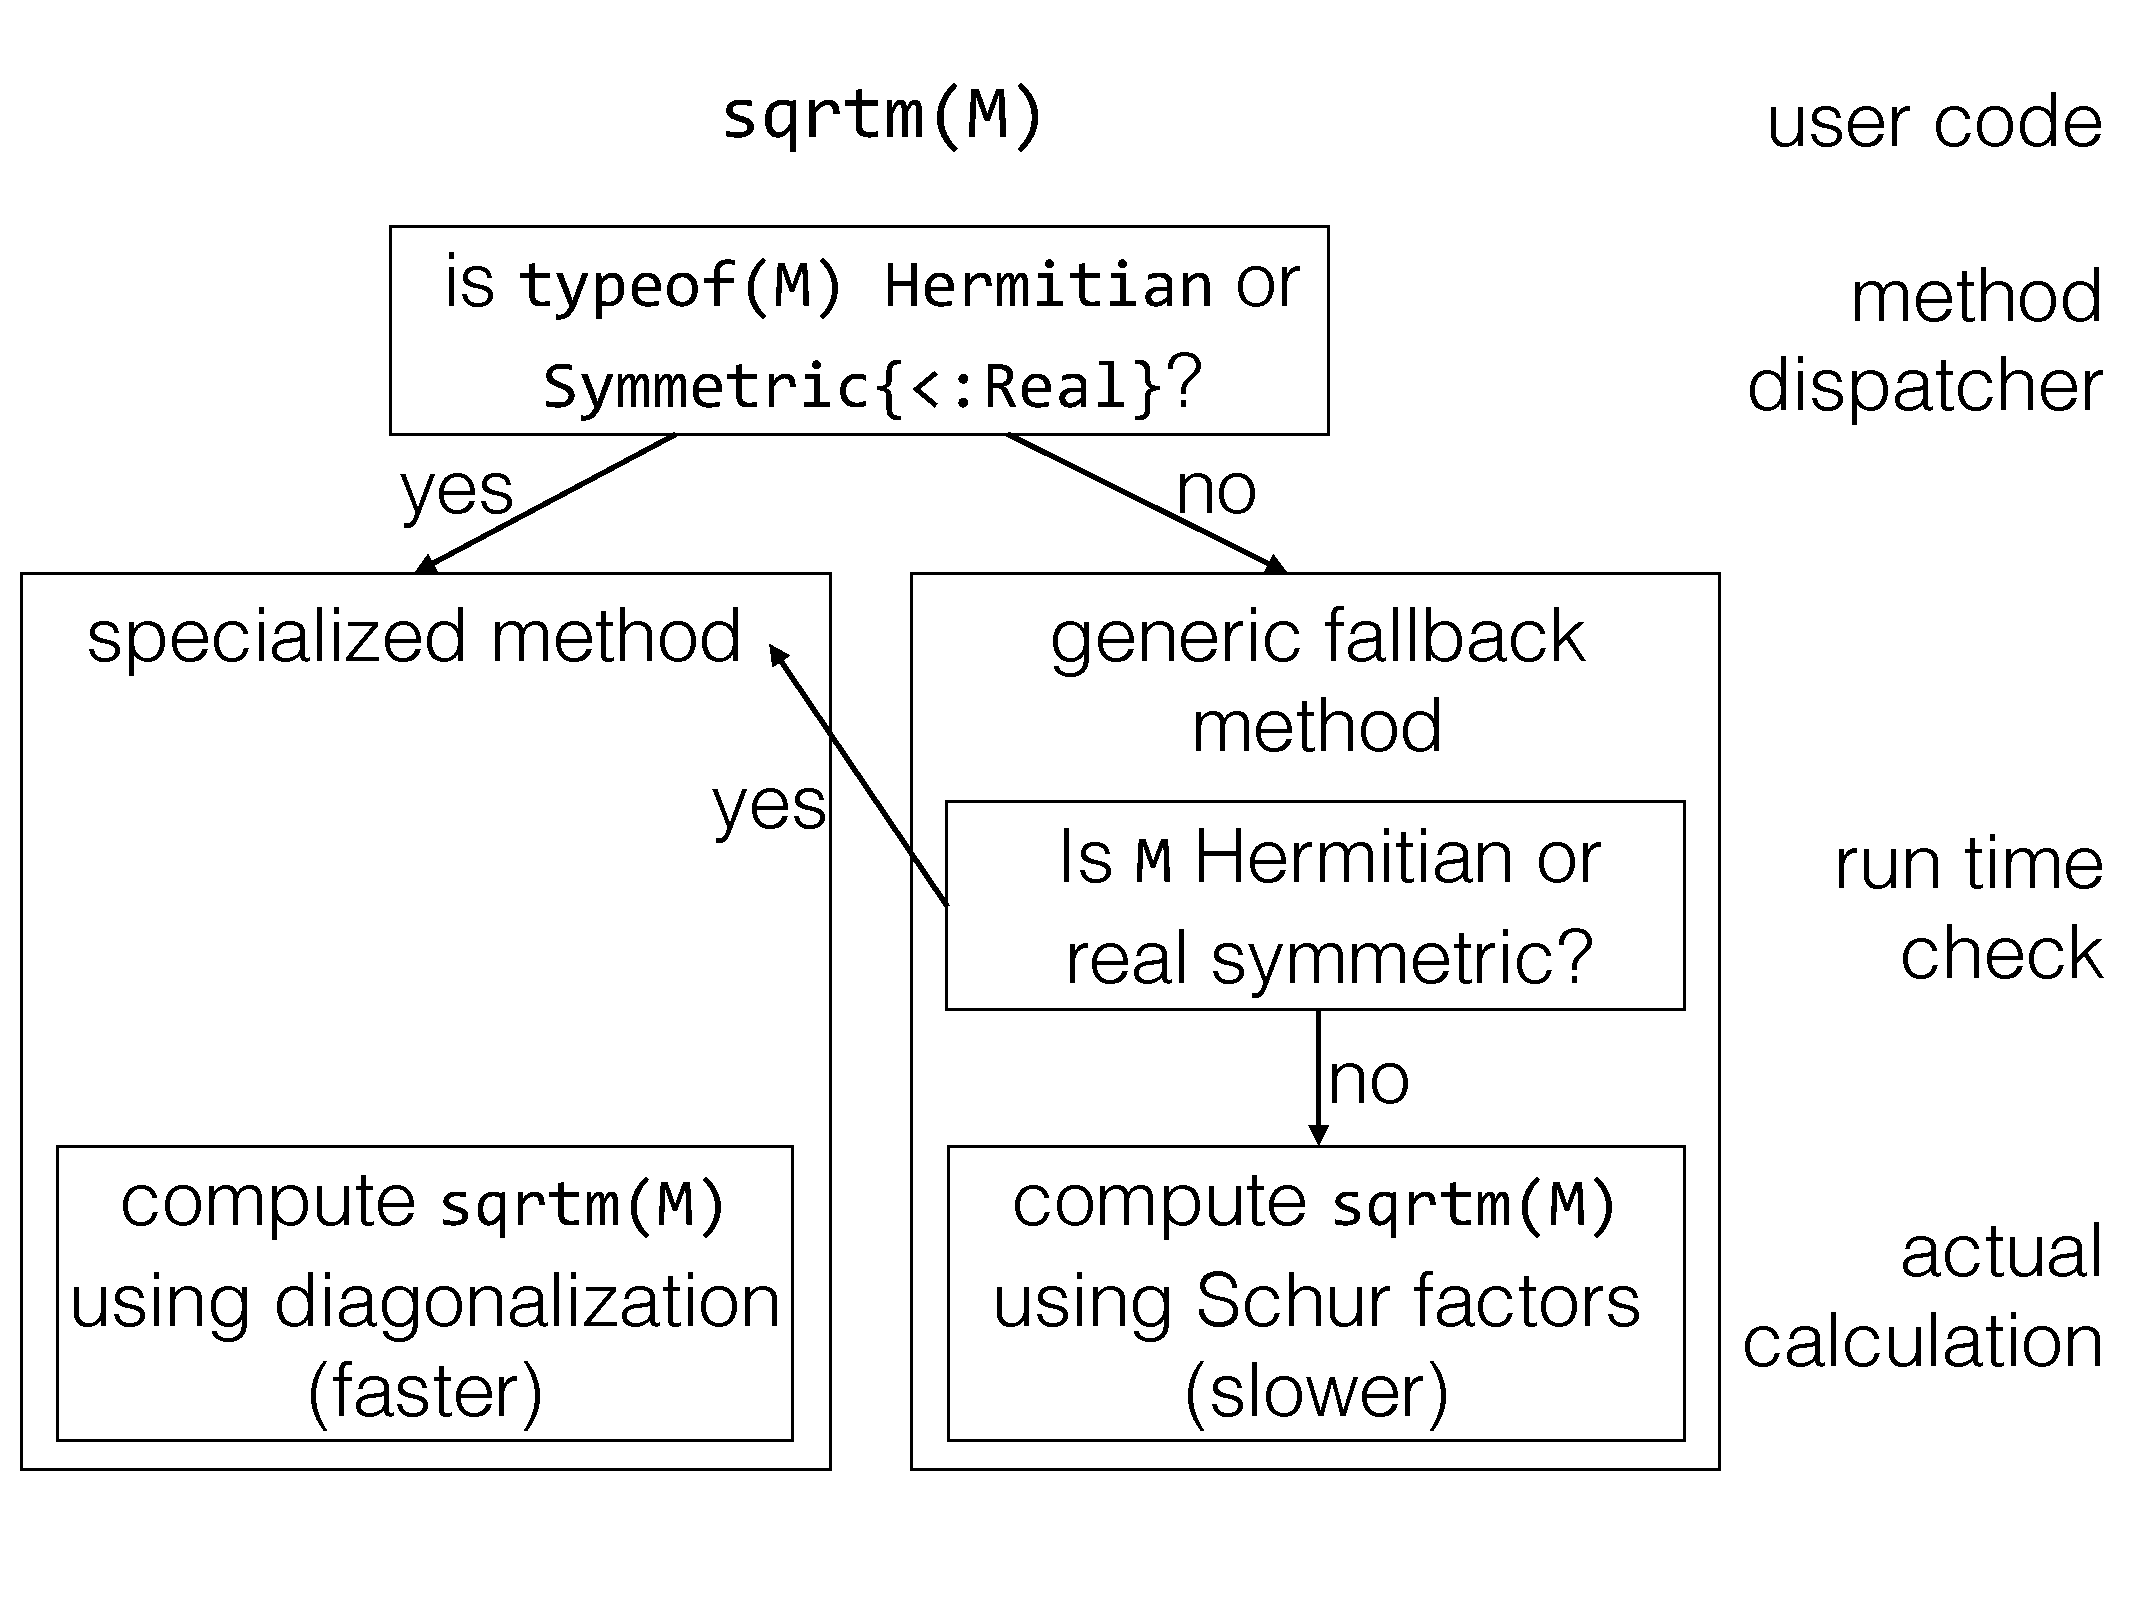
\includegraphics[width=\columnwidth]{fig-sqrtm}
	\caption{Dynamic dispatch and multimethods for the matrix square root
		function \texttt{sqrtm}, showing that the specialized algorithm
		can be run either from a static decision from the method
		dispatcher based on the input type, or a dynamic decision from
		a run-time check based on the value.}
	\label{fig:sqrtm}
\end{figure}

This modest example illustrates a pattern characteristic of technical
computing environments: dynamic dispatch on top of statically-typed
performance kernels.
However the difference here is that both components can be expressed
in the same language, and with the same notation.

In general, this is the kind of programming experience provided by
optimized implementations of dynamic languages, which can generate
code based on run time information.
However, code specialization is only half of the story.
The other half is extensibility --- adding new data types and
method definitions.
Julia's approach to extensibility is designed to take advantage of
specialization, by allowing methods to be defined for combinations
of structured types.


%The first code snippet illustrates a situation that can be addressed by either
%static dispatch or dynamic dispatch. However, the second snippet makes use of
%dynamic dispatch semantics to reuse code for the special case, if at run time
%the input was determined to satisfy the conditions of the special case.
%If we
%only had static dispatch, we would either have to forgo the
%specialized algorithm, or otherwise repeat that code in the general method.
%Therefore, dynamic dispatch allows for greater code reuse, allowing for greater
%overall performance without redundant code.


\subsection{Polymorphic types in Julia}

The method shown above demonstrates two kinds of polymorphism supported in
Julia. First, the input \lstinline|A| is annotated (\lstinline|::|) with the
type \lstinline|StridedMatrix|, which is an abstract type, not a concrete type.
A strided matrix is one that has a Fortran-compatible storage format, i.e.\ it
is stored in a contiguous block of memory and whose dimensions can be described
by a dope vector. The subtypes of \lstinline|StridedMatrix| in the base
library are \lstinline|Matrix| (ordinary matrices), and subarray types defining
views into strided matrices, whose referenced elements may not be fully
contiguous in memory. Thus, this \lstinline|sqrtm| method would be
dispatched upon by both \lstinline|Matrix| objects and subarrays, by virtue of
both types being subtypes of \lstinline|StridedMatrix|.

The second kind of polymorphism shown by the signature
\lstinline|sqrtm{T<:Real}(A::Matrix{T})| is parametric polymorphism. This
signature defines a family of related methods, one for each kind of
\lstinline|Matrix| containing a numeric type \lstinline|T| that is a subtype
(\lstinline|<:|) of \lstinline|Real|. This definition encompasses separate
definitions for matrices of type \lstinline|Matrix{Int32}| (matrices of 32-bit
integers), \lstinline|Matrix{Float64}| (matrices of 64-bit floating point real
numbers), and even \lstinline|Matrix{Rational{BigInt}}| (matrices of rational
numbers where the numerators and denominators are arbitrary precision
integers). Matrices containing other types, such as
\lstinline|Matrix{Complex{Float64}}|, would not dispatch on this family of methods.

The two kinds of polymorphism allow families of related methods to be defined
concisely, which allow highly generic code to be written. Additionally, code for
multiple algorithms can coexist within the same generic function, with the actual
choice of which code to run being determined by method dispatch. Furthermore,
the same performant kernel can be called even in situations where the user does
not know that a particular input matrix is symmetric, or even that specialized
algorithms for symmetric matrices exist.

